\documentclass[11pt]{article}
\usepackage[margin=0.9in]{geometry}
\usepackage{amsmath,amssymb}
\usepackage{booktabs}
\usepackage{graphicx}
\usepackage{fancyhdr}
\usepackage[hidelinks]{hyperref}

\graphicspath{{Figures/}}
\pagestyle{fancy}
\fancyhf{}
\lhead{STAT 546 \textbar{} HW7 implementation report \textbar{} Anurag Ramesh}
\rhead{17 November 2026}
\cfoot{\thepage}
\renewcommand{\headrulewidth}{0.4pt}
\setlength{\headheight}{14pt}
\setlength{\parindent}{0pt}
\setlength{\parskip}{6pt}

\newcommand{\E}{\mathbb{E}}
\newcommand{\Var}{\operatorname{Var}}

\begin{document}

All code is in \texttt{Scripts/}, one script per question, with \texttt{data.py} (Q1, Q2) and
\texttt{large\_model.py} (Q3) for the shared data. SGLD and SGHMC are in the root module
\path{Stochastic_Gradient_MCMC.py}; the full-data reference uses \path{Metropolis_Hastings.py}. Each script
saves its figure in \texttt{Figures/} and its numbers in \texttt{Results/}. CPU time is process time of the
sampling loop on one BLAS thread. Repeating an identical run changed it by up to 70\% on this machine, so
single CPU times are approximate.

\section*{Q1. SGLD for Bayesian logistic regression}

\subsection*{Model and gradient}

For $Y_i\in\{0,1\}$ with $P(Y_i=1\mid x_i,\theta)=s(x_i^T\theta)$, $s(z)=1/(1+e^{-z})$, and the prior
$\theta\sim N(0,\sigma_0^2I)$, the log posterior and its gradient are
\[
\log\pi(\theta)=\text{const}-\frac{\|\theta\|^2}{2\sigma_0^2}+\sum_{i=1}^N\left[Y_ix_i^T\theta-\log\left(1+e^{x_i^T\theta}\right)\right],
\qquad
\nabla\log\pi(\theta)=-\frac{\theta}{\sigma_0^2}+\sum_{i=1}^N\left(Y_i-s(x_i^T\theta)\right)x_i .
\]
With a minibatch $B$ of $b$ indices drawn uniformly with replacement,
\[
\hat g(\theta)=-\frac{\theta}{\sigma_0^2}+\frac Nb\sum_{i\in B}\left(Y_i-s(x_i^T\theta)\right)x_i
\]
is unbiased, $\E[\hat g(\theta)]=\nabla\log\pi(\theta)$, because each draw has expectation
$\frac1N\sum_i(Y_i-s(x_i^T\theta))x_i$. Its variance is
$V(\theta)=\frac{N^2}{b}\Var_i\!\left[(Y_i-s(x_i^T\theta))x_i\right]$, which falls as $1/b$.

\subsection*{From Langevin dynamics to SGLD}

The Langevin diffusion $d\theta_t=\frac12\nabla\log\pi(\theta_t)\,dt+dW_t$ has $\pi$ as its stationary
distribution. Its Fokker--Planck equation is
\[
\partial_t p=-\nabla\cdot\left(\tfrac12p\nabla\log\pi\right)+\tfrac12\Delta p,
\]
and at $p=\pi$ the drift term is $-\frac12\nabla\cdot\nabla\pi=-\frac12\Delta\pi$, which cancels the diffusion term.
An Euler step of length $\epsilon$ gives
$\theta_{t+1}=\theta_t+\frac{\epsilon}{2}\nabla\log\pi(\theta_t)+N(0,\epsilon I)$. MALA would accept or
reject this with a Metropolis--Hastings step, which needs the full data. SGLD (Welling and Teh, 2011)
drops that step and replaces the gradient with $\hat g$:
\[
\boxed{\;\theta_{t+1}=\theta_t+\frac{\epsilon_t}{2}\hat g(\theta_t)+\xi_t,\qquad \xi_t\sim N(0,\epsilon_tI)\;}
\]
Each step costs $O(bd)$ instead of $O(Nd)$.

\textbf{Why the gradient noise matters.} The step contains the gradient error
$\frac{\epsilon_t}{2}(\hat g-\nabla\log\pi)$, with variance $\epsilon_t^2V/4$, next to the injected noise of
variance $\epsilon_t$. Their ratio $\epsilon_tV/4$ goes to 0 as $\epsilon_t\to0$. With steps satisfying
$\sum_t\epsilon_t=\infty$ and $\sum_t\epsilon_t^2<\infty$, averages weighted by $\epsilon_t$,
$\sum_t\epsilon_tf(\theta_t)/\sum_t\epsilon_t$, are consistent (Teh, Thiery and Vollmer, 2016). With a
constant step the noise does not vanish. Near the mode, write $\log\pi$ as locally quadratic with precision
$\lambda_j$ in coordinate $j$, and treat the coordinates as roughly independent. Then
$\theta'_j-m_j=(1-\epsilon\lambda_j/2)(\theta_j-m_j)+\text{noise}$ with noise variance
$\epsilon+\epsilon^2V_j/4$. The stationary variance $\sigma_j^2$ solves
$\sigma_j^2=(1-\epsilon\lambda_j/2)^2\sigma_j^2+\epsilon+\epsilon^2V_j/4$, so
\[
\frac{\text{SGLD standard deviation}}{\text{posterior standard deviation}}
\approx\sqrt{\frac{1+\epsilon V_j/4}{1-\epsilon\lambda_j/4}} .
\]
The numerator is the inflation caused by gradient noise; the denominator is the discretization bias, which
remains even with the full gradient.

\subsection*{Data, reference and settings}

I simulated $N=5{,}000$ training and 5,000 test observations with an intercept and 9 independent $N(0,1)$
predictors, true coefficients $(-0.5,1,-1,0.5,-0.5,0.25,-0.25,0,0,0)$, and prior variance $\sigma_0^2=10$ (seed
546). The full-data reference is random-walk Metropolis--Hastings on the exact posterior, with a normal
proposal of covariance $(2.38^2/d)\hat H^{-1}$ (Roberts, Gelman and Gilks, 1997), where $\hat H$ is the
Hessian of $-\log\pi$ at the mode. It ran 200,000 iterations, discarded 10,000, accepted 26.5\% of proposals and
took 79 CPU seconds. Its effective sample size was at least 5,565 for every coefficient, so its Monte Carlo
error is about 1.3\% of a posterior standard deviation.

Every SGLD run starts at $\theta=0$, runs 50,000 iterations and discards the first 5,000 (seed 548). I
report the posterior mean error,
$\sqrt{\frac1d\sum_j\left((\hat m_j-m_j)/s_j\right)^2}$, in units of the reference standard deviations $s_j$;
the average ratio $\hat s_j/s_j$ of estimated to reference standard deviations; and the first iteration at
which every coordinate is within $3s_j$ of the reference mean. The prediction uses $V_j$ measured at the mode
and $\lambda_j=1/s_j^2$.

\subsection*{Results}

The decreasing sequence is $\epsilon_t=5\times10^{-4}(1+t/1000)^{-0.55}$, which falls to
$5.8\times10^{-5}$ by the end. ``Reached'' is the first iteration within $3s_j$ of the reference mean in every
coordinate.

\begin{center}
\begin{tabular}{llcccc}
\toprule
\textbf{Study} & \textbf{Setting} & \textbf{Mean error} & \textbf{SD ratio} & \textbf{Predicted} & \textbf{Reached} \\
\midrule
Minibatch size & $b=10$ & 0.425 & 3.35 & 3.37 & 86 \\
($\epsilon=10^{-4}$) & $b=100$ & 0.051 & 1.40 & 1.43 & 68 \\
 & $b=1{,}000$ & 0.028 & 1.05 & 1.06 & 88 \\
 & $b=5{,}000$ (all data) & 0.035 & 1.00 & 1.01 & 73 \\
\midrule
Step size & $\epsilon=2\times10^{-5}$ & 0.091 & 1.06 & 1.10 & 355 \\
($b=100$) & $\epsilon=10^{-4}$ & 0.051 & 1.40 & 1.43 & 68 \\
 & $\epsilon=5\times10^{-4}$ & 0.186 & 2.56 & 2.59 & 19 \\
 & decreasing & 0.054 & 1.40 & -- & 19 \\
\bottomrule
\end{tabular}
\end{center}

\textbf{Minibatch size.} Small minibatches inflate the posterior spread: $b=10$ gives standard deviations 3.35
times too large, and its mean error is 0.43 posterior standard deviations. The inflation shrinks as $b$
grows, and with all the data only the discretization bias remains (ratio 1.00). The prediction above matches
every constant-step run to within 4\%.

\textbf{Step size.} A larger step reaches the posterior sooner (19 iterations at $5\times10^{-4}$, 355 at
$2\times10^{-5}$) but inflates the spread more. The smallest step has an accurate spread but moves slowly, so
after 45,000 kept iterations its mean is still 0.09 standard deviations off. The decreasing sequence starts
fast. Its step-weighted averages still give a ratio of 1.40 after 50,000 iterations, because the early, larger
steps carry the most weight; the theory is asymptotic.

All runs had test accuracy between 0.760 and 0.761, the same as the reference (0.761), even with three-fold
inflation: predictive accuracy here says little about posterior accuracy.

\begin{center}
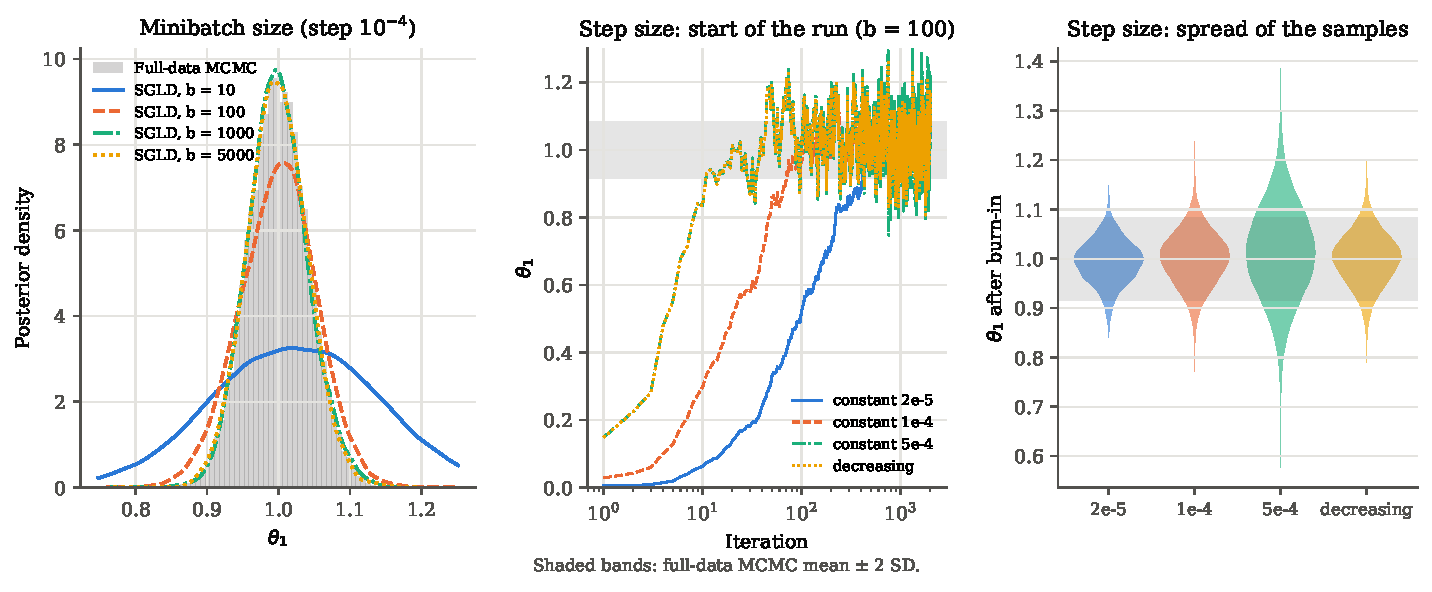
\includegraphics[width=\textwidth]{q1_sgld.pdf}
\end{center}
{\small All runs share the same random numbers, so the decreasing sequence, which starts at
$5\times10^{-4}$, follows the $5\times10^{-4}$ path early on.}

\newpage
\section*{Q2. SGHMC}

\subsection*{Derivation}

Write $U(\theta)=-\log\pi(\theta)$.

\textbf{Momentum.} Introduce an auxiliary momentum $r\in\mathbb R^d$ with $r\sim N(0,M)$, independent of
$\theta$, and the Hamiltonian $H(\theta,r)=U(\theta)+\frac12r^TM^{-1}r$. The joint density
$\pi(\theta,r)\propto e^{-H(\theta,r)}$ has $\theta$-marginal $\pi$. Hamilton's equations
\[
d\theta=M^{-1}r\,dt,\qquad dr=-\nabla U(\theta)\,dt
\]
keep $H$ constant and preserve volume, so they leave $e^{-H}$ invariant. The momentum carries $\theta$ in a
consistent direction over many steps instead of the random-walk behaviour of Langevin dynamics.

\textbf{Noisy gradients add energy.} With a minibatch gradient $\nabla\tilde U=-\hat g$, a step of length
$\epsilon$ changes $r$ by $-\epsilon\nabla\tilde U\approx-\epsilon\nabla U+N(0,\epsilon^2V)$. In continuous time
this is $dr=-\nabla U\,dt+N(0,2B\,dt)$ with $B=\frac12\epsilon V$. Nothing removes the energy this noise adds,
so $e^{-H}$ is no longer stationary, and the chain drifts away from the posterior (Chen, Fox and Guestrin,
2014).

\textbf{Friction and compensating noise.} SGHMC adds a friction term $-CM^{-1}r$ that removes energy, and
injects Gaussian noise $N(0,2(C-\hat B)dt)$, where $\hat B$ estimates the gradient-noise term $B$. When
$\hat B=B$, the total noise is exactly $2C$, matching the friction:
\[
d\theta=M^{-1}r\,dt,\qquad dr=-\nabla U(\theta)\,dt-CM^{-1}r\,dt+N(0,2C\,dt).
\]
These are underdamped Langevin dynamics, for which $e^{-H}$ is stationary (Chen et al., 2014, verify this
with the Fokker--Planck equation). The friction must exceed the gradient noise, $C\succeq\hat B$.

\textbf{Discretization.} With $v=\epsilon M^{-1}r$, learning rate $\eta=\epsilon^2M^{-1}$, friction
$\alpha=\epsilon M^{-1}C$ and $\hat\beta=\epsilon M^{-1}\hat B=\frac12\eta\hat V$ (unit mass), the Euler steps
become
\[
\boxed{\;\theta_{t+1}=\theta_t+v_t,\qquad
v_{t+1}=(1-\alpha)v_t+\eta\,\hat g(\theta_{t+1})+N\!\left(0,\,2(\alpha-\hat\beta)\eta I\right)\;}
\]
This is SGD with momentum plus calibrated noise. With $\alpha=1$ the momentum is discarded each step and
$\theta_{t+1}=\theta_t+\eta\hat g+N(0,2\eta I)$, which is SGLD with $\epsilon=2\eta$. Heavy friction
therefore turns SGHMC into SGLD with step $2\eta/\alpha$. I estimated $\hat V_j$, the variance of the
minibatch gradient, at the posterior mode from 2,000 minibatch gradients (0.1 CPU seconds); $\hat\beta=0$
ignores it.

\subsection*{Comparison with SGLD}

Both samplers use the Q1 data and minibatch size 100, and run 50,000 iterations with the first 5,000
discarded. Each setting was repeated with 5 seeds, and the table gives means. Across seeds, ESS and ESS/s
varied by up to about 25\% of their means, the mean error by up to about 35\%, and the SD ratio by about 1\%. ESS is ArviZ's effective sample size, minimum and median
over the 10 coefficients; ESS/s is the median ESS per CPU second; ``corr.'' means $\hat\beta=\eta\hat V/2$.

\begin{center}
\small
\setlength{\tabcolsep}{5pt}
\begin{tabular}{lccccc}
\toprule
\textbf{Sampler} & \textbf{CPU (s)} & \textbf{ESS min/med} & \textbf{ESS/s} & \textbf{Mean error} & \textbf{SD ratio} \\
\midrule
SGLD, $\epsilon=2\times10^{-5}$ & 1.82 & 106 / 167 & 93 & 0.086 & 1.085 \\
SGLD, $\epsilon=10^{-4}$ & 1.60 & 608 / 921 & 589 & 0.053 & 1.412 \\
SGHMC, $\eta=10^{-5}$, $\alpha=0.3$, $\hat\beta=0$ & 1.75 & 396 / 598 & 345 & 0.053 & 1.278 \\
SGHMC, $\eta=10^{-5}$, $\alpha=0.3$, corr. & 1.85 & 420 / 608 & 330 & 0.046 & 0.980 \\
SGHMC, $\eta=2\times10^{-6}$, $\alpha=0.05$, corr. & 1.80 & 494 / 658 & 369 & 0.042 & 0.978 \\
\bottomrule
\end{tabular}
\end{center}

\textbf{Cost.} One iteration of either sampler evaluates one minibatch gradient, so the CPU times are the
same within timing noise. For comparison, the full-data reference used 79 CPU seconds.

\textbf{Efficiency at equal accuracy.} The corrected SGHMC runs have standard deviations about 2\% below the
reference. The SGLD run with an accurate spread ($\epsilon=2\times10^{-5}$, ratio 1.085) has a median ESS of
167, while SGHMC with $\eta=2\times10^{-6}$, $\alpha=0.05$ has 658, about four times as many in the same CPU
time. The autocorrelation of $\theta_1$ falls to zero in about 100 iterations for SGHMC and about 500--600 for
SGLD. SGLD can reach a similar ESS only with a larger step, $\epsilon=10^{-4}$, which inflates the spread by
41\%.

\textbf{The compensating noise.} With $\hat\beta=0$, SGHMC inflates the spread by 28\%. Setting
$\hat\beta=\eta\hat V/2$ (at most 0.23 here, below $\alpha=0.3$) removes the inflation at no loss of ESS. Test
accuracy was 0.761 in every run.

\begin{center}
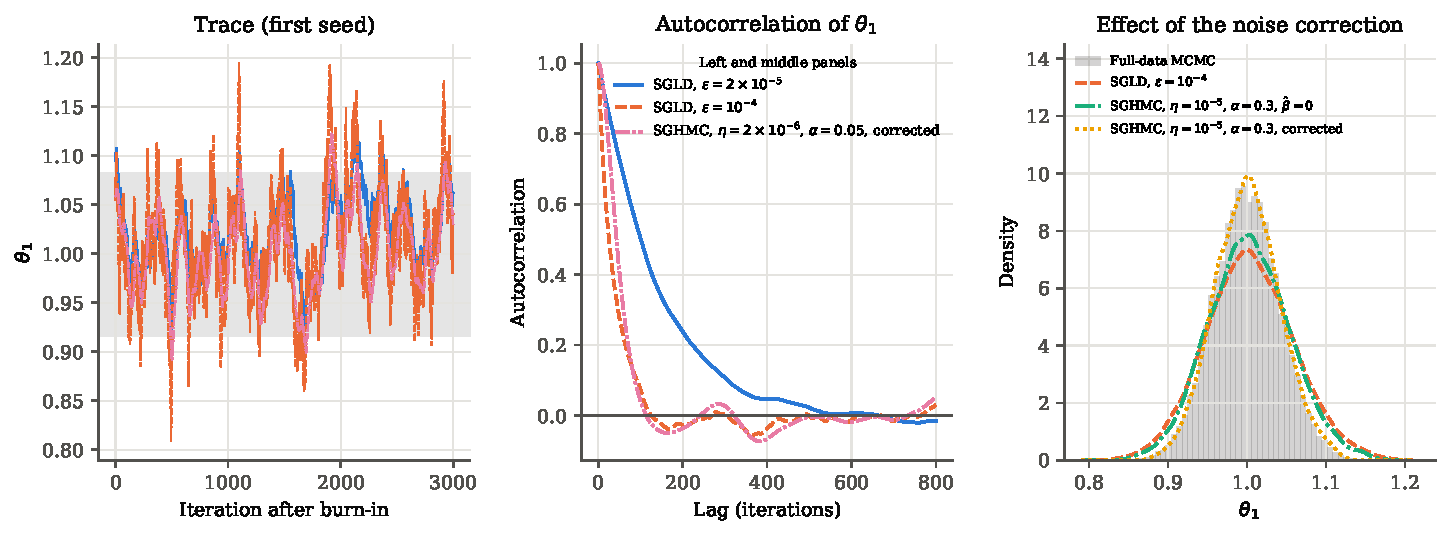
\includegraphics[width=\textwidth]{q2_sghmc.pdf}
\end{center}

\newpage
\section*{Q3. Numerical study on a larger model}

\subsection*{Model and measures}

The model is a Bayesian linear regression with $N=100{,}000$ training and 20,000 test observations and
$d=100$ predictors:
\[
y_i=x_i^T\beta+e_i,\qquad e_i\sim N(0,1),\qquad \beta\sim N(0,I),\qquad x_i\sim N(0,\Sigma_x),\ (\Sigma_x)_{jk}=0.5^{|j-k|},
\]
with the true coefficients drawn from $N(0,0.5^2)$ (seed 546). The noise variance is treated as known, so the
posterior is exactly $N(m,S)$ with $S=(X^TX+I)^{-1}$ and $m=SX^Ty$. Posterior estimation error is therefore
measured against the exact answer. The posterior standard deviations are 0.0037--0.0041.

For each run I report CPU time, the minimum and median ESS over the 100 coefficients, the posterior mean error
and SD ratio as in Q1 (now against the exact $m$ and $\sqrt{S_{jj}}$), and predictive accuracy as the excess
test RMSE of $x^T\hat m$ over $x^Tm$ (the exact posterior mean gives test RMSE 0.99980).

The baseline is $b=1{,}000$ and 20,000 iterations, with the first 10\% discarded, for both samplers; SGLD uses
$\epsilon=6\times10^{-7}$, and SGHMC uses $\eta=3\times10^{-9}$, $\alpha=0.01$, $\hat\beta=0$. At this scale
the gradient noise is large, and keeping $\hat\beta=\eta\hat V/2$ below $\alpha$ forced very small learning
rates; in trial runs where $\hat\beta$ was close to $\alpha$ the spread became too small (ratio 0.82). I
therefore used $\hat\beta=0$ in this study. Each study changes one factor, using seed 21. Runs were
sequential.

\subsection*{Results}

\begin{center}
\small
\setlength{\tabcolsep}{2.5pt}
\begin{tabular}{llccccc}
\toprule
\textbf{Study} & \textbf{Run} & \textbf{CPU (s)} & \textbf{ESS min/med} & \textbf{Mean error} & \textbf{SD ratio} & \textbf{RMSE excess} \\
 & & & & & & ($\times10^{-5}$) \\
\midrule
Batch size & SGLD, $b=100$ & 1.9 & 60 / 163 & 0.297 & 3.20 & 10.0 \\
 & SGLD, $b=1{,}000$ & 13.1 & 60 / 149 & 0.133 & 1.38 & 1.7 \\
 & SGLD, $b=10{,}000$ & 147.4 & 31 / 127 & 0.106 & 1.05 & -1.4 \\
 & SGHMC, $b=100$ & 1.2 & 87 / 121 & 0.273 & 3.18 & 7.9 \\
 & SGHMC, $b=1{,}000$ & 14.9 & 83 / 106 & 0.110 & 1.36 & 1.9 \\
 & SGHMC, $b=10{,}000$ & 146.0 & 37 / 96 & 0.091 & 1.04 & 5.4 \\
\midrule
Learning rate & SGLD, $\epsilon=2\times10^{-7}$ & 11.0 & 15 / 49 & 0.195 & 1.12 & 1.1 \\
 & SGLD, $\epsilon=6\times10^{-7}$ & 9.9 & 60 / 149 & 0.133 & 1.38 & 1.7 \\
 & SGLD, $\epsilon=2\times10^{-6}$ & 9.3 & 324 / 537 & 0.100 & 2.05 & 2.1 \\
 & SGHMC, $\eta=10^{-9}$ & 9.3 & 6 / 42 & 0.162 & 1.13 & 1.7 \\
 & SGHMC, $\eta=3\times10^{-9}$ & 8.8 & 83 / 106 & 0.110 & 1.36 & 1.9 \\
 & SGHMC, $\eta=10^{-8}$ & 9.8 & 211 / 236 & 0.085 & 1.99 & 2.1 \\
\midrule
Friction & SGHMC, $\alpha=0.003$ & 9.1 & 121 / 137 & 0.086 & 2.04 & 2.4 \\
($\eta=3\times10^{-9}$) & SGHMC, $\alpha=0.01$ & 7.9 & 83 / 106 & 0.110 & 1.36 & 1.9 \\
 & SGHMC, $\alpha=0.03$ & 7.7 & 6 / 45 & 0.161 & 1.13 & 1.6 \\
 & SGHMC, $\alpha=0.1$ & 7.4 & 2 / 12 & 0.462 & 1.42 & -0.3 \\
\bottomrule
\end{tabular}
\end{center}

\begin{center}
\small
\setlength{\tabcolsep}{4pt}
\begin{tabular}{lcccccccc}
\toprule
& \multicolumn{4}{c}{\textbf{SGLD}} & \multicolumn{4}{c}{\textbf{SGHMC}} \\
\cmidrule(lr){2-5}\cmidrule(lr){6-9}
\textbf{Iter.} & CPU & ESS min/med & Error & SD ratio & CPU & ESS min/med & Error & SD ratio \\
\midrule
2,500 & 1.0 & 2 / 20 & 0.368 & 1.46 & 1.0 & 8 / 16 & 1.107 & 5.33 \\
5,000 & 2.1 & 3 / 38 & 0.243 & 1.38 & 1.9 & 6 / 30 & 0.271 & 1.67 \\
10,000 & 4.1 & 6 / 71 & 0.171 & 1.39 & 3.8 & 7 / 53 & 0.144 & 1.36 \\
20,000 & 8.2 & 60 / 149 & 0.133 & 1.38 & 7.6 & 83 / 106 & 0.110 & 1.36 \\
50,000 & 20.5 & 249 / 352 & 0.081 & 1.39 & 19.0 & 214 / 263 & 0.083 & 1.38 \\
\bottomrule
\end{tabular}
\end{center}
{\small The iteration study uses prefixes of one 50,000-iteration run per sampler (first 10\% of each prefix
discarded), with its CPU time prorated.}

\begin{center}
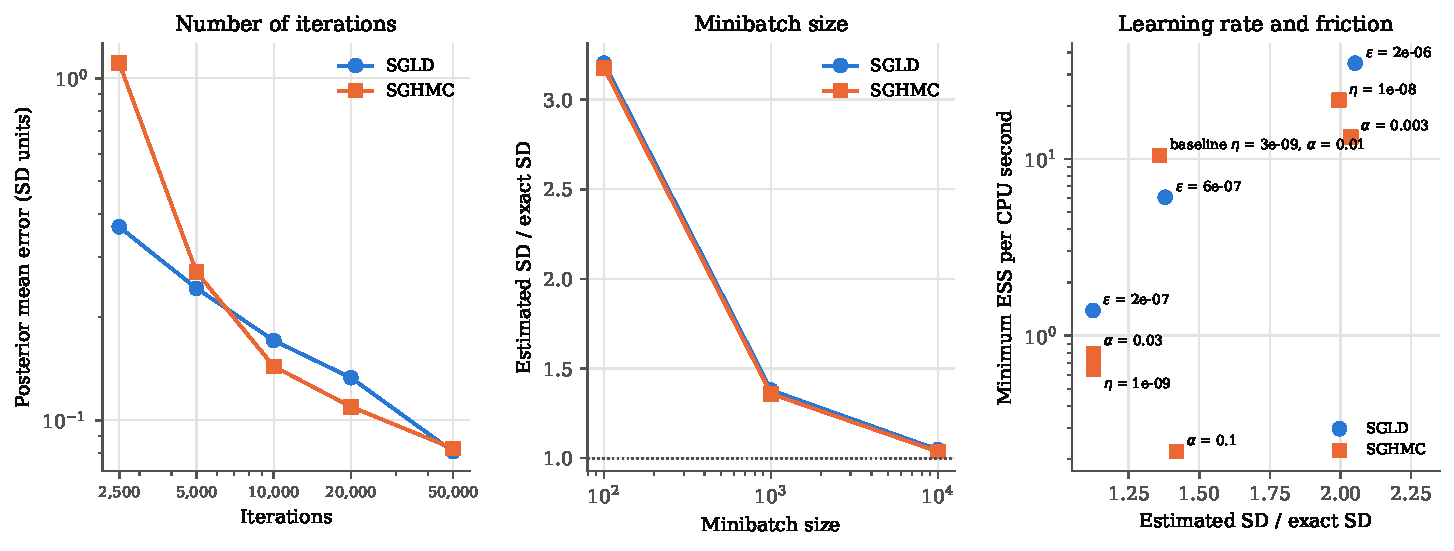
\includegraphics[width=\textwidth]{q3_study.pdf}
\end{center}

\subsection*{Discussion}

\textbf{Minibatch size.} This controls the bias. For both samplers the SD ratio falls from about 3.2 at
$b=100$ to 1.04--1.05 at $b=10{,}000$, but the larger batches cost 75--120 times as much CPU time for the same
number of iterations.

\textbf{Learning rate.} This trades mixing against bias. Raising $\epsilon$ from $2\times10^{-7}$ to
$2\times10^{-6}$ increases SGLD's minimum ESS from 15 to 324 but inflates the spread from 1.12 to 2.05. SGHMC
behaves the same way as $\eta$ changes.

\textbf{Friction.} Low friction keeps more momentum and mixes faster ($\alpha=0.003$: minimum ESS 121), but
with $\hat\beta=0$ nothing then damps the gradient noise, and the spread doubles. High friction removes the
momentum: $\alpha=0.03$ with $\eta=3\times10^{-9}$ gives almost exactly the same results as $\alpha=0.01$ with
$\eta=10^{-9}$, as the limit $\epsilon=2\eta/\alpha$ predicts, and $\alpha=0.1$ barely moves in 20,000
iterations (minimum ESS 2).

\textbf{Number of iterations.} More iterations reduce the Monte Carlo error: the mean error falls roughly
like $T^{-1/2}$, from about 0.17 at 10,000 iterations to 0.08 at 50,000. They do not reduce the bias: the SD
ratio stays near 1.38 from 10,000 to 50,000 iterations for both samplers. SGHMC with low friction also needs a
longer burn-in: its 2,500-iteration prefix still contains the initial transient (SD ratio 5.3).

\textbf{Predictive accuracy.} Excess test RMSE was at most $10^{-4}$ (against an RMSE of 1.0) in every run of
the first table, including runs with a three-fold inflated spread; the largest value in the iteration study
was $8.6\times10^{-4}$, for the 2,500-iteration SGHMC prefix. As in Q1 and Q2, prediction from the posterior mean is
insensitive to errors in posterior uncertainty, so it cannot replace a direct check of the posterior.

\textbf{SGLD versus SGHMC.} In this well-conditioned model, momentum gave no consistent advantage. At a
similar SD ratio of about 1.37, SGHMC had the higher minimum ESS (83 against 60) but the lower median (106
against 149). At about 2.0, SGLD had the higher ESS. In Q2, with the noise correction, SGHMC was about four
times as efficient at equal accuracy.

\textbf{Strengths.} Both samplers cost $O(bd)$ per iteration, independent of $N$, and both are a few lines
of code on top of minibatch gradients.

\textbf{Limitations.}
\begin{itemize}
\item Neither has a Metropolis--Hastings correction, so with constant steps both have a bias that more
iterations do not remove. Only smaller steps or larger batches reduce it.
\item SGLD is a random walk, which is slow in poorly scaled directions.
\item SGHMC can move faster through momentum, but has more to tune: $\eta$, $\alpha$ and $\hat\beta$. Its
noise correction is valuable when $\hat\beta$ can be kept well below $\alpha$ (Q2), and fragile when it
cannot (Q3).
\end{itemize}

\newpage
\section*{Saved results}

\texttt{q1\_reference\_mcmc.npz} holds the full-data MCMC samples. \texttt{q1.json} and \texttt{q2.json} hold
every run's measures, including each of the five Q2 seeds and the estimated gradient-noise variances.
\texttt{q3.json} holds every Q3 run.

\section*{References}
\sloppy

STAT 546, Fall 2026. Homework 7, Questions 1--3. The problems and requested methods are taken from the assignment.

M. Welling and Y. W. Teh (2011). Bayesian learning via stochastic gradient Langevin dynamics. In
\emph{Proceedings of the 28th International Conference on Machine Learning}, 681--688.

T. Chen, E. Fox and C. Guestrin (2014). Stochastic gradient Hamiltonian Monte Carlo. In \emph{Proceedings of
the 31st International Conference on Machine Learning}, PMLR 32(2), 1683--1691.

Y. W. Teh, A. H. Thiery and S. J. Vollmer (2016). Consistency and fluctuations for stochastic gradient Langevin
dynamics. \emph{Journal of Machine Learning Research}, 17(7), 1--33.

G. O. Roberts, A. Gelman and W. R. Gilks (1997). Weak convergence and optimal scaling of random walk Metropolis
algorithms. \emph{The Annals of Applied Probability}, 7(1), 110--120.
DOI: \href{https://doi.org/10.1214/aoap/1034625254}{10.1214/aoap/1034625254}.

\end{document}
